\newpage


\section{Results}\label{sec:results}
This sections presents the measurement and visualization graphs of the proposed solution.

\afterpage{%
    \clearpage% Flush earlier floats (otherwise order might not be correct)
    \begin{landscape}% Landscape page
        \begin{figure}
            \centering
            \subfloat{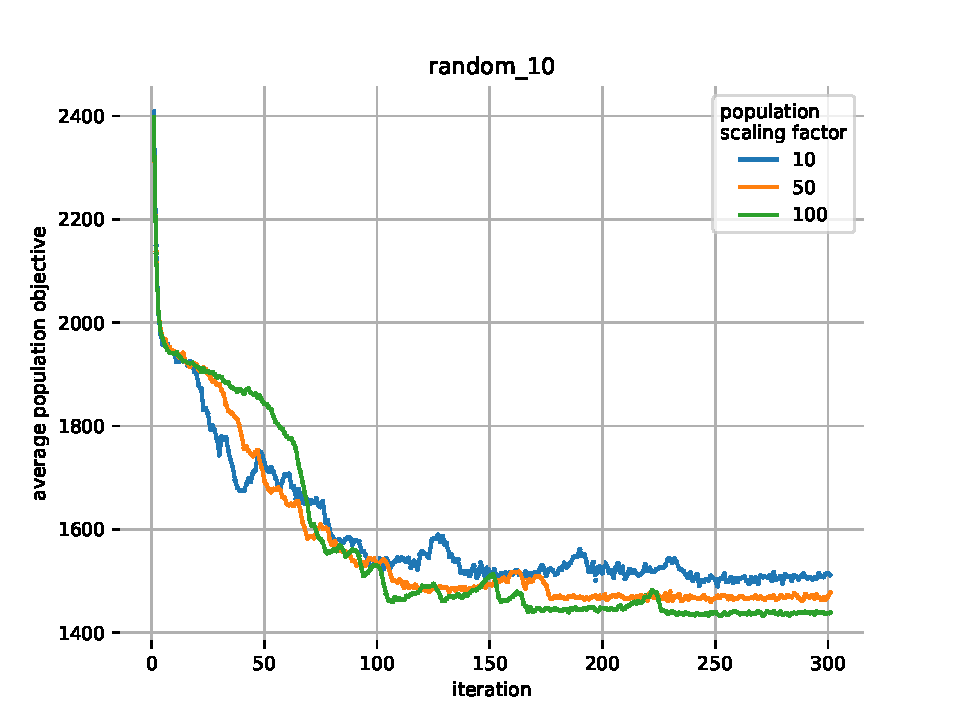
\includegraphics[width=0.8\textwidth]{pop_size_random_10}\label{subfig:pop-size-random-10}}
            \subfloat{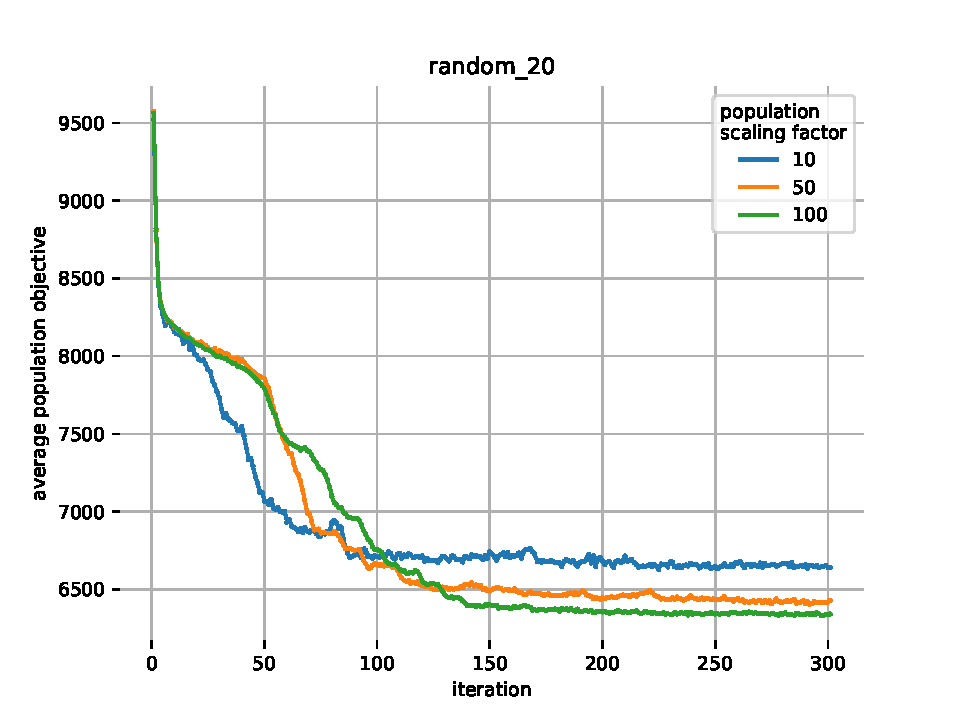
\includegraphics[width=0.8\textwidth]{pop_size_random_20}\label{subfig:pop-size-random-20}}
            \caption[Testing population scaling factor]
            {Testing population scaling factor at two random instances.
            For population scaling factor $k$ and instance of size $N$, i.e. the number of paintings, population size is $kN$.}
            \label{fig:pop-size}%
        \end{figure}
    \end{landscape}
    \clearpage% Flush page
}

\afterpage{%
    \clearpage% Flush earlier floats (otherwise order might not be correct)
    \begin{landscape}% Landscape page
        \begin{figure}
            \centering
            \subfloat{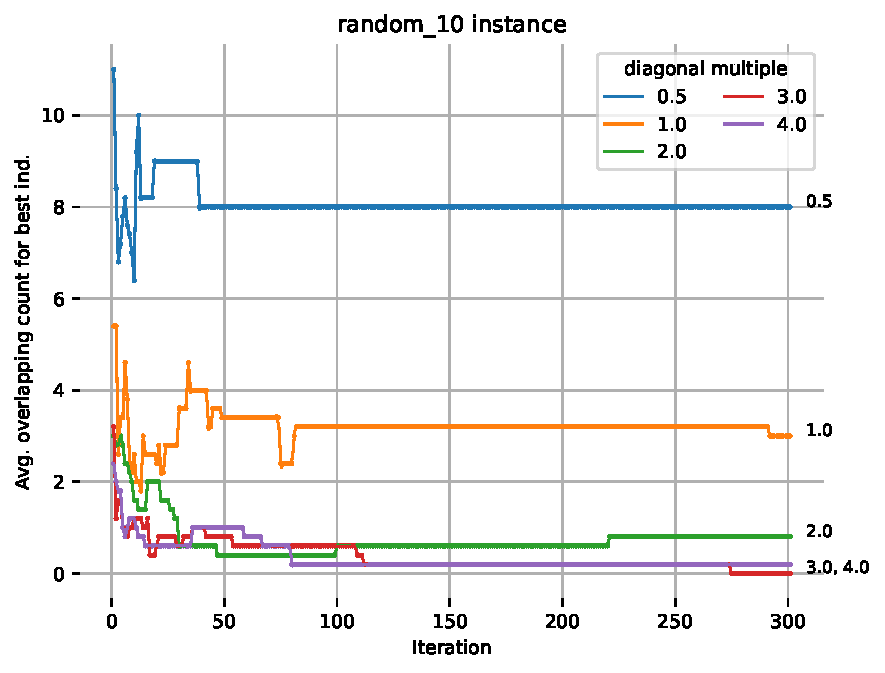
\includegraphics[width=0.8\textwidth]{overlapping_penalization_constant_random_10}\label{subfig:overlapping-random-10}}
            \subfloat{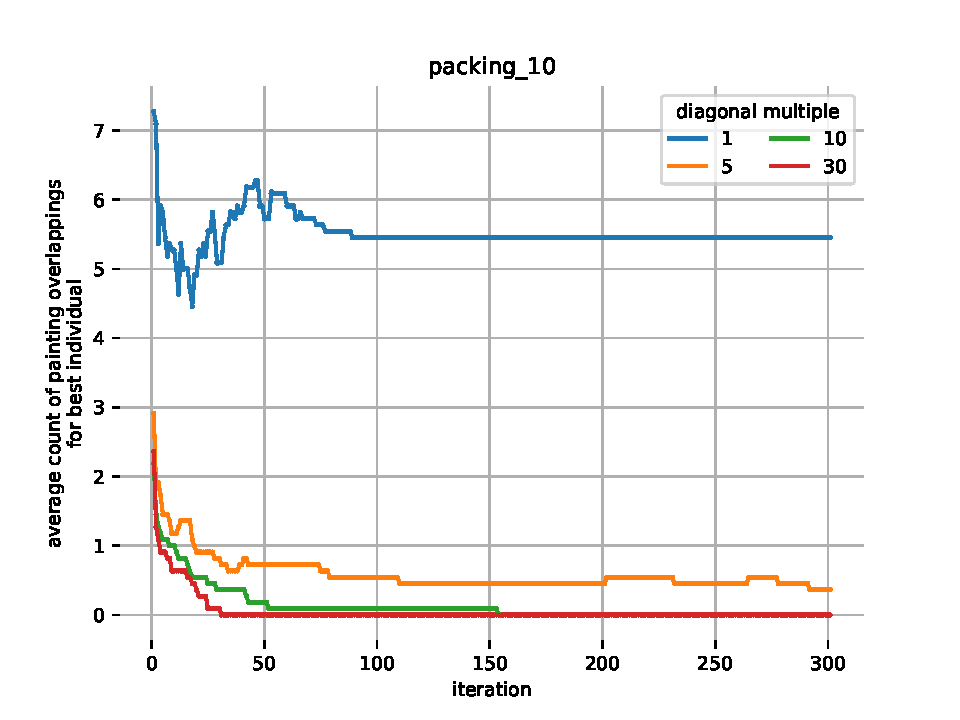
\includegraphics[width=0.8\textwidth]{overlapping_penalization_constant_packing_10}\label{subfig:overlapping-packing-10}}
            \caption[Testing population overlapping penalization constant]
            {Testing overlapping penalization contanst.
            Diagonal multiple $k$ determines overlapping penalization constant as $k\sqrt{w^2 + h^2}$, where $w$, $h$ are dimension of the layout.}
            \label{fig:overlapping-penalization}%
        \end{figure}
    \end{landscape}
    \clearpage% Flush page
}

\afterpage{%
    \clearpage% Flush earlier floats (otherwise order might not be correct)
    \begin{landscape}% Landscape page
        \begin{figure}
            \centering
            \subfloat{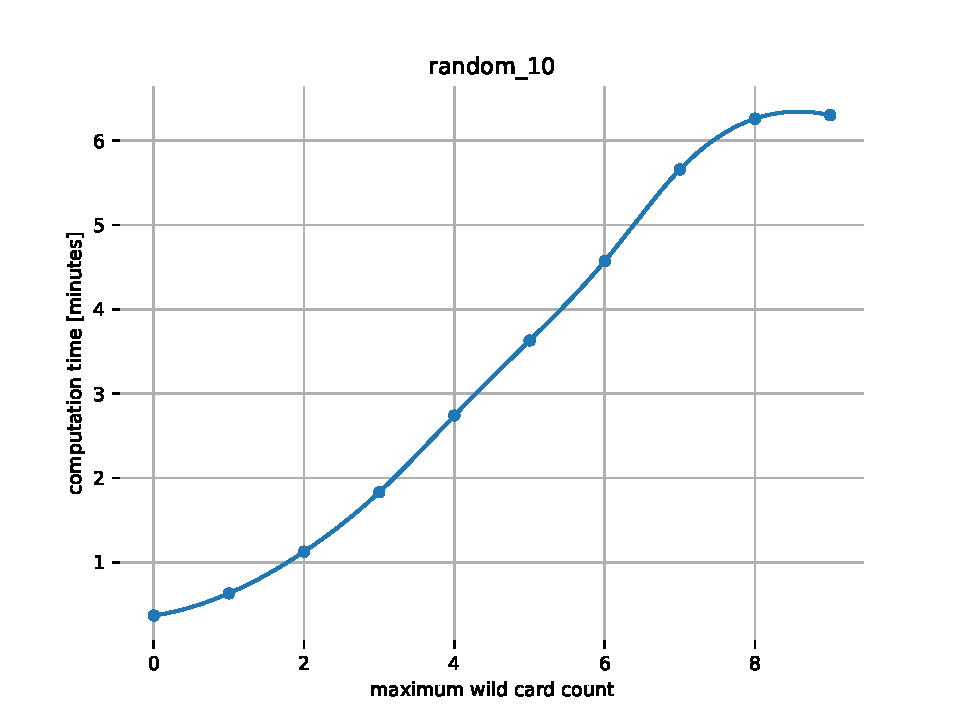
\includegraphics[width=0.8\textwidth]{computation_time_random_10}\label{subfig:computation-time-10}}
%            \subfloat{\includegraphics[width=0.8\textwidth]{computation_time_random_20}\label{subfig:computation-time-20}}
            \caption[Testing computation speed]
            {Testing computation speed for increasing maximum wild card count.}
            \label{fig:computation-time}%
        \end{figure}
    \end{landscape}
    \clearpage% Flush page
}

\afterpage{%
    \clearpage% Flush earlier floats (otherwise order might not be correct)
    \begin{landscape}% Landscape page
        \begin{figure}
            \centering
            \subfloat{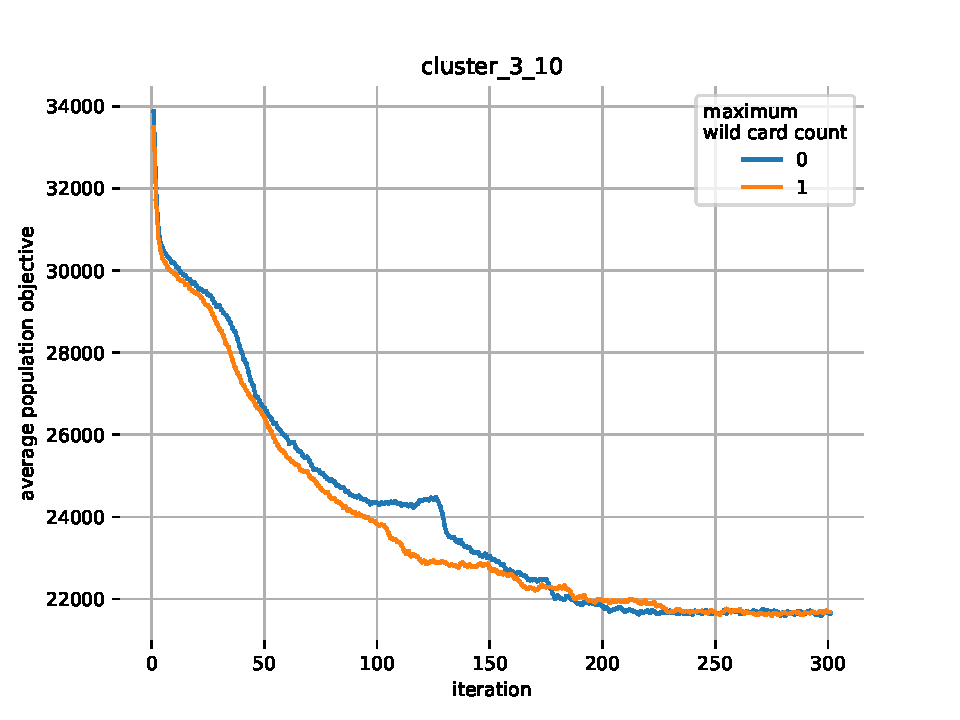
\includegraphics[width=0.8\textwidth]{cluster_3_10}\label{subfig:cluster-3-10}}
            \subfloat{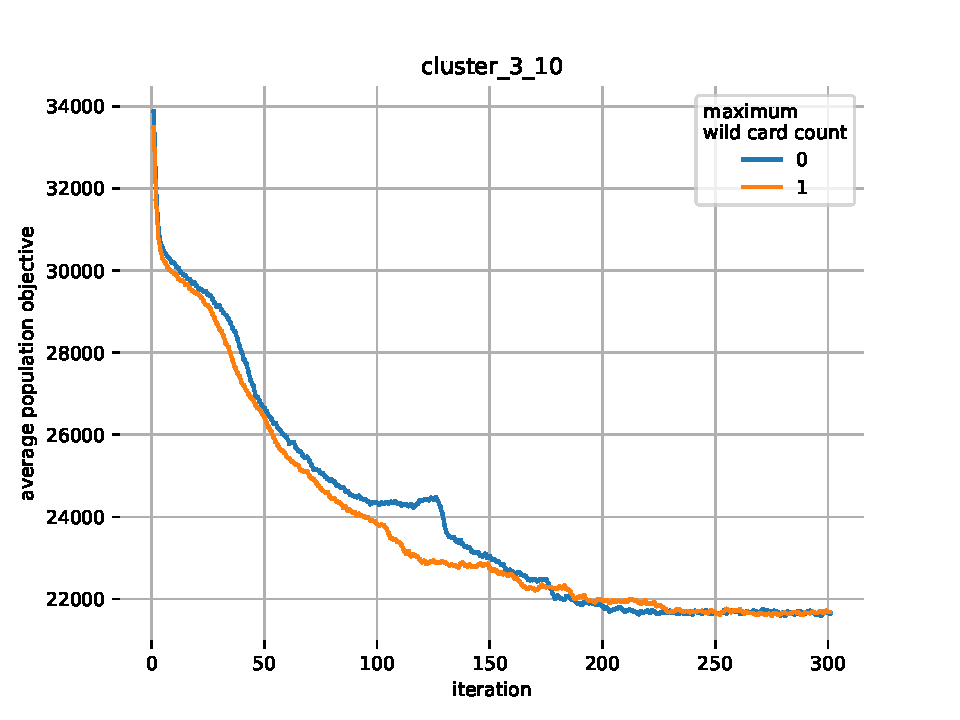
\includegraphics[width=0.8\textwidth]{cluster_3_10}\label{subfig:cluster-3-10}}
            \caption[Testing clustering dataset]
            {Testing clustering dataset performance with a different maximum wildcard count.}
            \label{fig:cluster}%
        \end{figure}
    \end{landscape}
    \clearpage% Flush page
}

\afterpage{%
    \clearpage% Flush earlier floats (otherwise order might not be correct)
    \begin{landscape}% Landscape page
        \begin{figure}
            \centering
            \subfloat[brute-force]{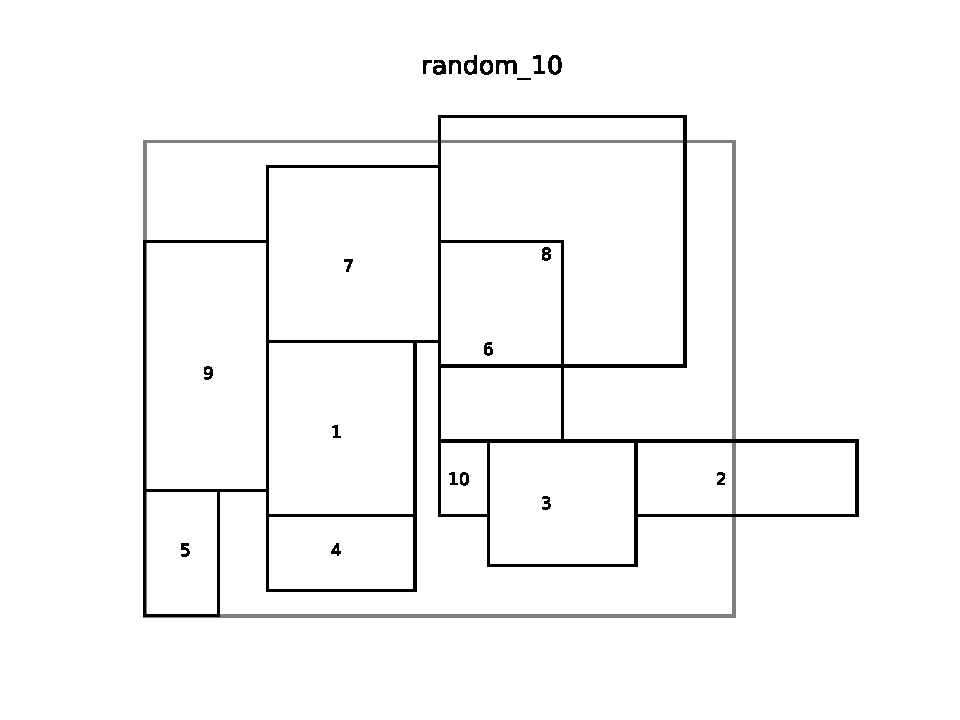
\includegraphics[width=0.9\textwidth]{visualization_random10_brute}\label{subfig:random10-brute}}
            \subfloat[proposed solution]{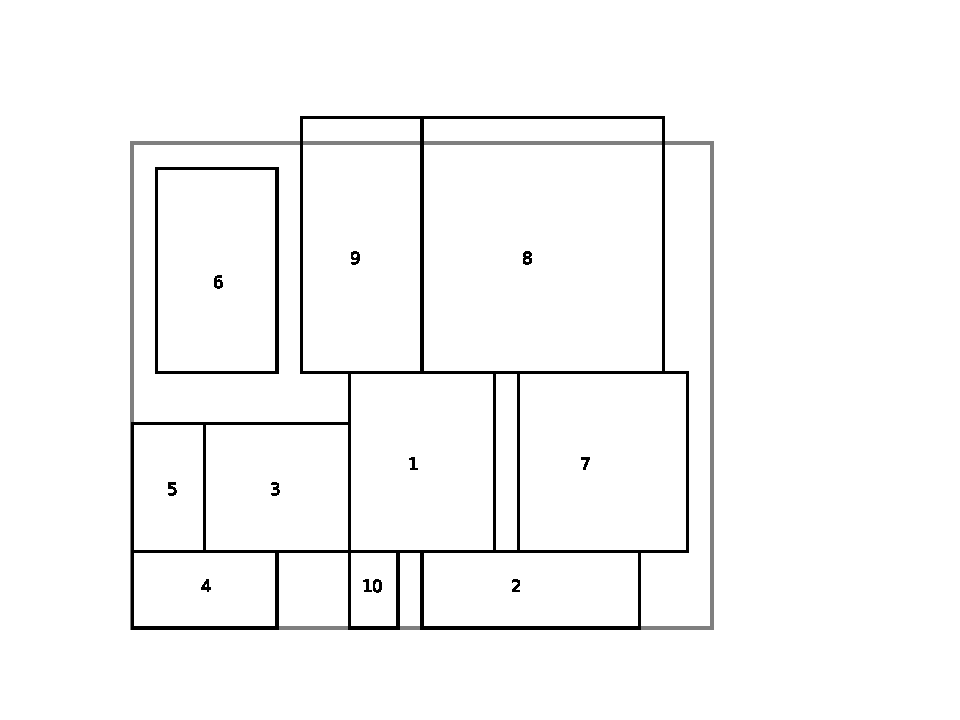
\includegraphics[width=0.9\textwidth]{visualization_random10_ga}\label{subfig:random10-ga}}
            \caption[Random\_10 instance solution visualization for brute-force]
                {Visualization of best result of proposed solution and brute-force for random\_10 instance.}
            \label{fig:visualization-random10}%
        \end{figure}
    \end{landscape}
    \clearpage% Flush page
}

\afterpage{%
    \clearpage% Flush earlier floats (otherwise order might not be correct)
    \begin{landscape}% Landscape page
        \begin{figure}
            \centering
            \subfloat[brute-force]{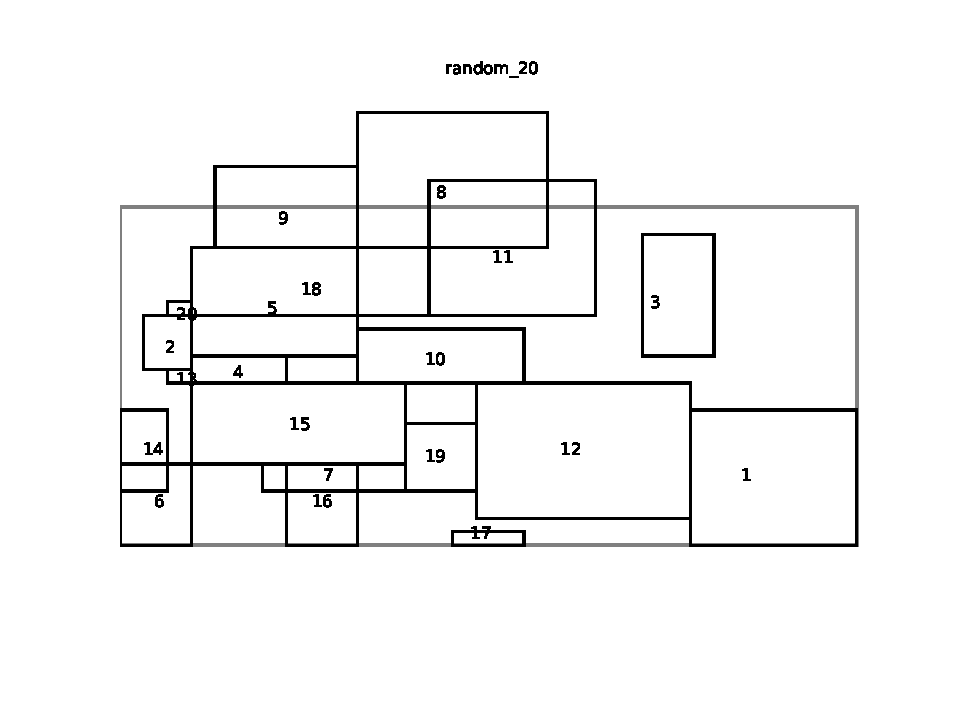
\includegraphics[width=0.8\textwidth]{visualization_random20_brute}\label{subfig:random20-brute}}
            \subfloat[proposed solution]{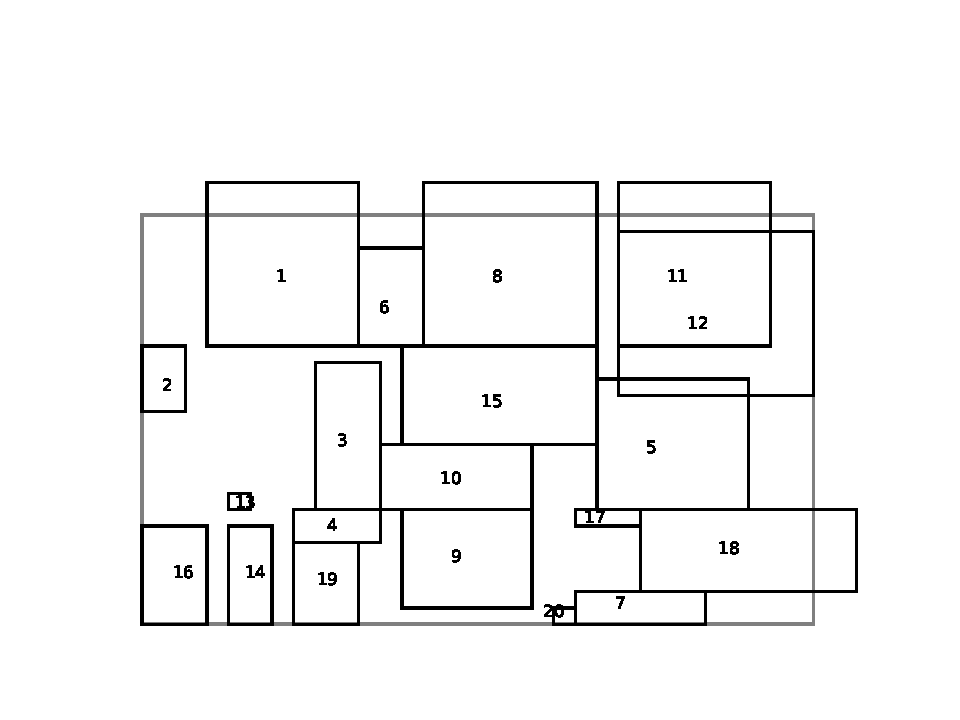
\includegraphics[width=0.8\textwidth]{visualization_random20_ga}\label{subfig:random20-ga}}
            \caption[Random\_10 instance solution visualization for proposed solution]
                {Visualization of best result of proposed solution and brute-force for random\_20 instance.}
            \label{fig:visualization-random20}%
        \end{figure}
    \end{landscape}
    \clearpage% Flush page
}

\afterpage{%
    \clearpage% Flush earlier floats (otherwise order might not be correct)
    \begin{landscape}% Landscape page
        \begin{figure}
            \centering
            \subfloat{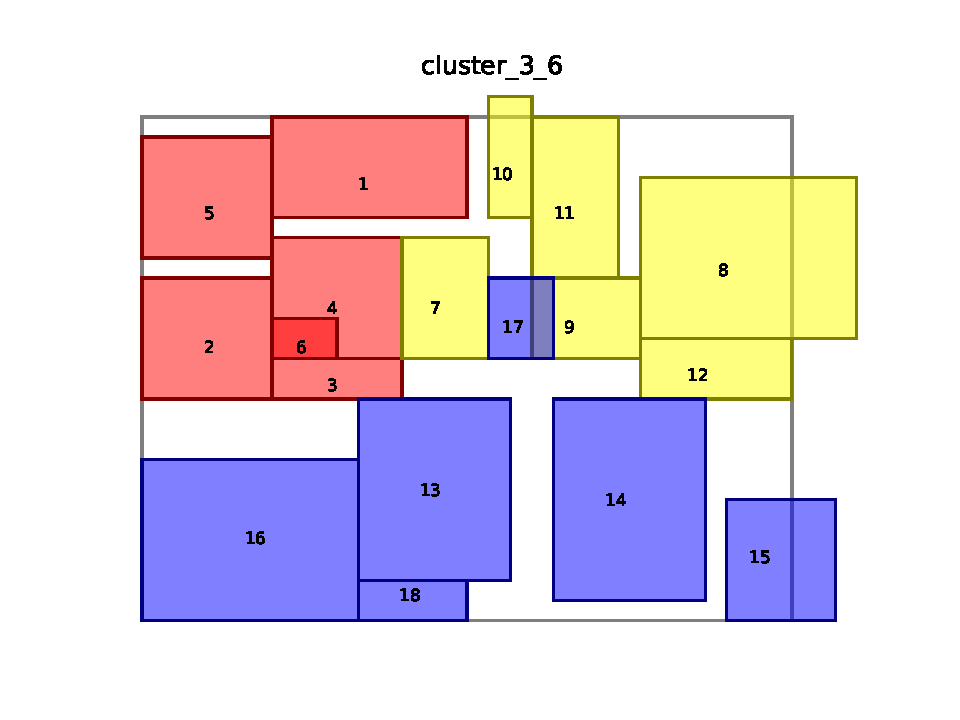
\includegraphics[width=0.8\textwidth]{visualization_cluster_3_6_ga}\label{subfig:cluster-3-6-ga}}
            \subfloat{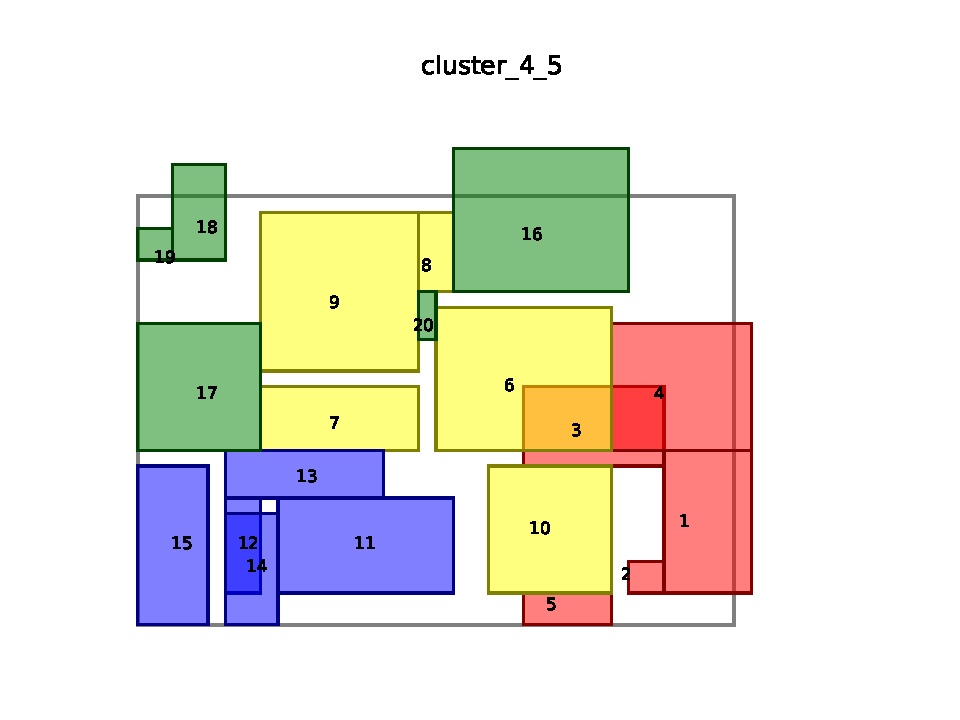
\includegraphics[width=0.8\textwidth]{visualization_cluster_4_5_ga}\label{subfig:cluster-4-5-ga}}
            \caption[Solution visualization of clustering instances for proposed solution]
            {Visualization of the best result of proposed solution for instances cluster\_3\_6 and cluster\_4\_5.}
            \label{fig:visualization-cluster}%
        \end{figure}
    \end{landscape}
    \clearpage% Flush page
}

\afterpage{%
    \clearpage% Flush earlier floats (otherwise order might not be correct)
    \begin{landscape}% Landscape page
        \begin{figure}
            \centering
            \subfloat{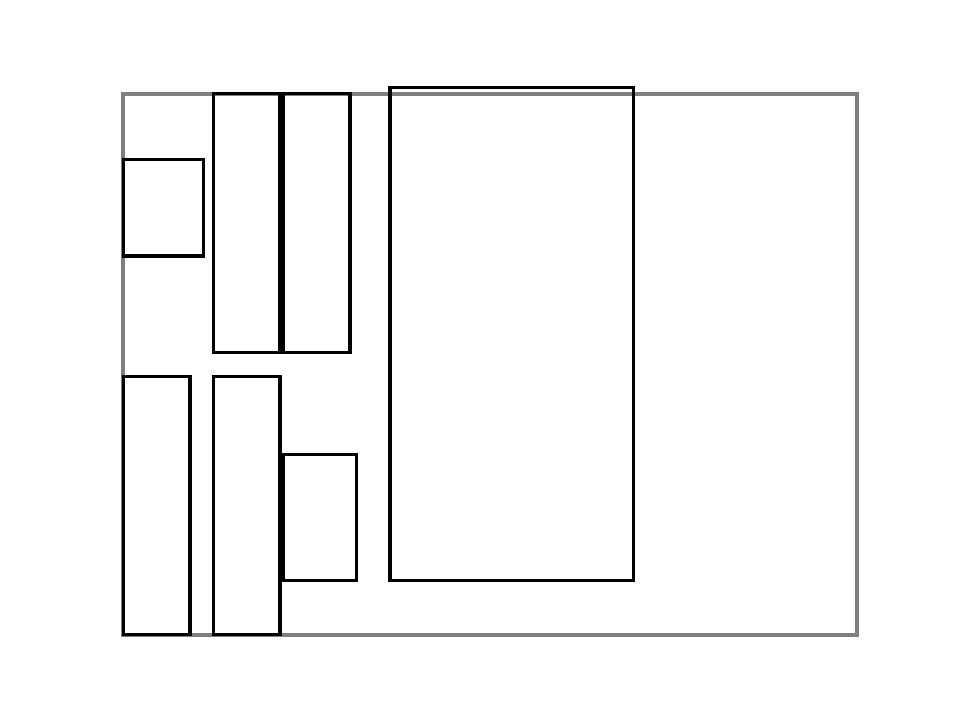
\includegraphics[width=0.8\textwidth]{visualization_london_nationa_gallery_ga}\label{subfig:london-gallery-ga}}
            \caption[London National Gallery solution visualization]
            {Visualization of the London National Gallery wall dataset.}
            \label{fig:visualization-cluster}%
        \end{figure}
    \end{landscape}
    \clearpage% Flush page
}
